% !TeX spellcheck = en_GB 
\section{Simulation}
In order to simulate interlocking structures with a range of design parameters we automatically generate an INP file in Abaqus CAE (2020) using a script.
Solving the INP file gives us the force-displacement graph, from which we can determine the ultimate tensile strength.
In order to simulate accurately we used the stress-strain curves from tensile tests on the base materials printed flat on the build plate as the plasticity in tabular form.
The simulations were performed in the Abaqus/Explicit solver where Dynamic,Explicit procedure step was used with the mass scaling factor of $10^7$,
using geometric nonlinearity and general contact (explicit) to disregard friction for simplicity.

The repeating nature of the interlocking patterns was captured by modelling half the geometry and apply symmetry constraints to the sides, top and bottom.
The model was meshed using C3D8R hexahedral elements of $\pm\SI{75}{\micro\meter}$.

A grid search was used to measure the influence on the ultimate strength along each of the design variables $\wb (,\va, \hc)$, along with the total length $\lmax$.
The simulation space was therefore 4D and 2D for the straight and diagonal design respectively.
In order to estimate the optimum we fit a smooth response surface to these data points using a radial basis function network,\cite{Dinh2002}
where a smoothness of $\lambda=1$ seemed to produce satisfactory results.


\subsection{Straight}
In order to prevent stress concentrations and adhere to manufacturing accuracy, the vertical edges of the straight design were rounded with $r=\SI{0.15}{\milli\meter}$;
see \cref{fig:sim_diagonal_model}.
We performed two rounds of hypersurface fitting on grid search; the second round was in a zoomed in region and with elements of $\pm\SI{50}{\micro\meter}$.

Newton's method was used to determine the optimum, starting from the best sampled point.
This step only considered the dimensions $\wb$ and $\va$, because $\lmax$ is given and $\hf$ has to be an integer multiple of $\hmin$.
It's unlikely the optimum of the fitted hypersurface would be on a different integer multiple of $\hmin$.
The resulting hypersurfaces are visualized in \cref{fig:simulation_results_straight}.
The obtained optima are shown in \cref{tab:sim_straight_optima}.

\begin{figure}
	\centering
	\begin{subfigure}[B]{.45\columnwidth}
		\centering
		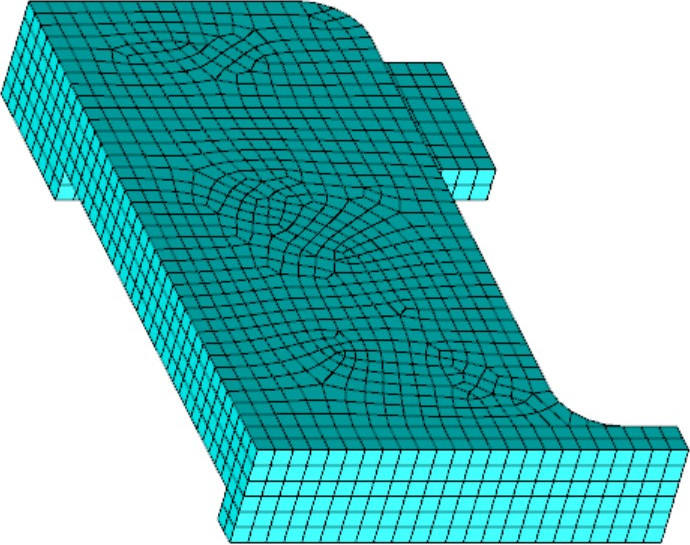
\includegraphics[width=\columnwidth]{sources/simulation/mesh-pp.jpg}
		\caption{PP}
	\end{subfigure}
	\begin{subfigure}[B]{.45\columnwidth}
		\centering
		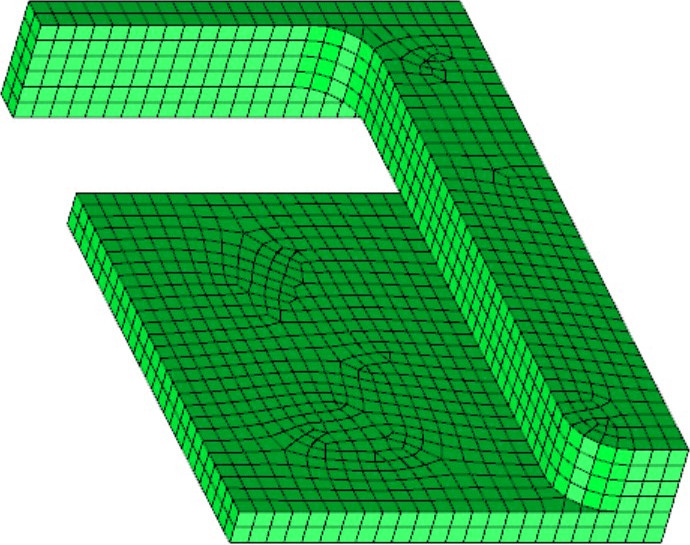
\includegraphics[width=\columnwidth]{sources/simulation/mesh-pla.jpg}
		\caption{TPLA}
	\end{subfigure}
	\caption{Example simulation mesh of the diagonal design.}
	\label{fig:sim_diagonal_model}
\end{figure}



\begin{figure*}
	\centering
	\begin{subfigure}[B]{.49\columnwidth}
		\centering
		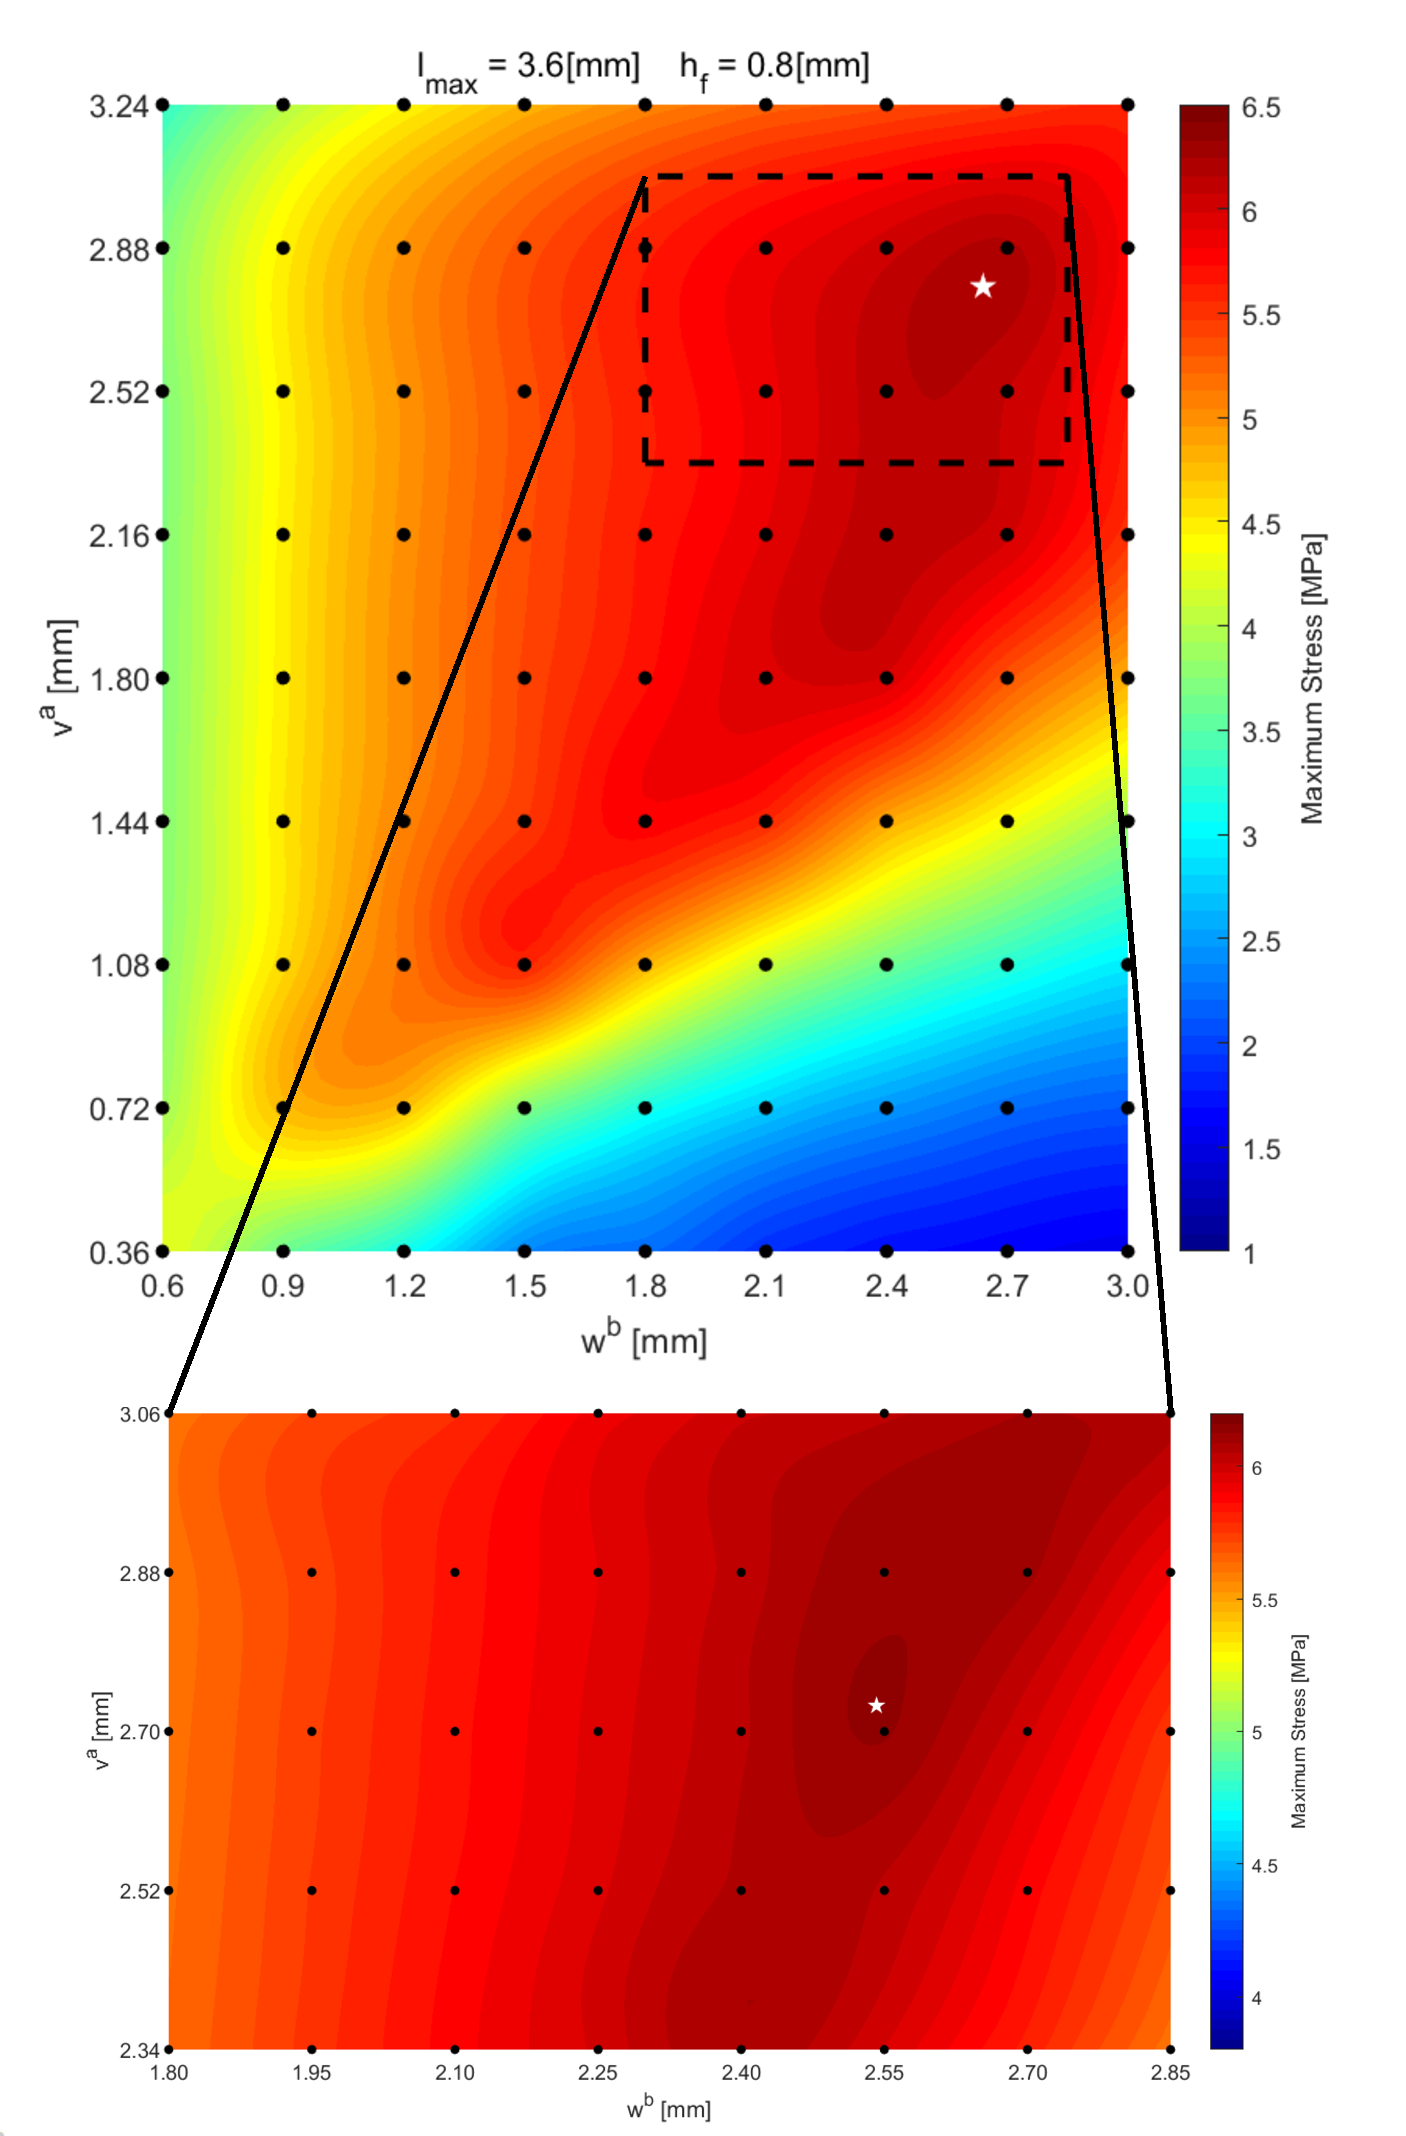
\includegraphics{sources/simulation/r12-lmax3.6.pdf}
		\caption{$\lmax=\SI{3.6}{\milli\meter}; \hf=\SI{0.8}{\milli\meter}$}
	\end{subfigure}
	\begin{subfigure}[B]{.49\columnwidth}
		\centering
		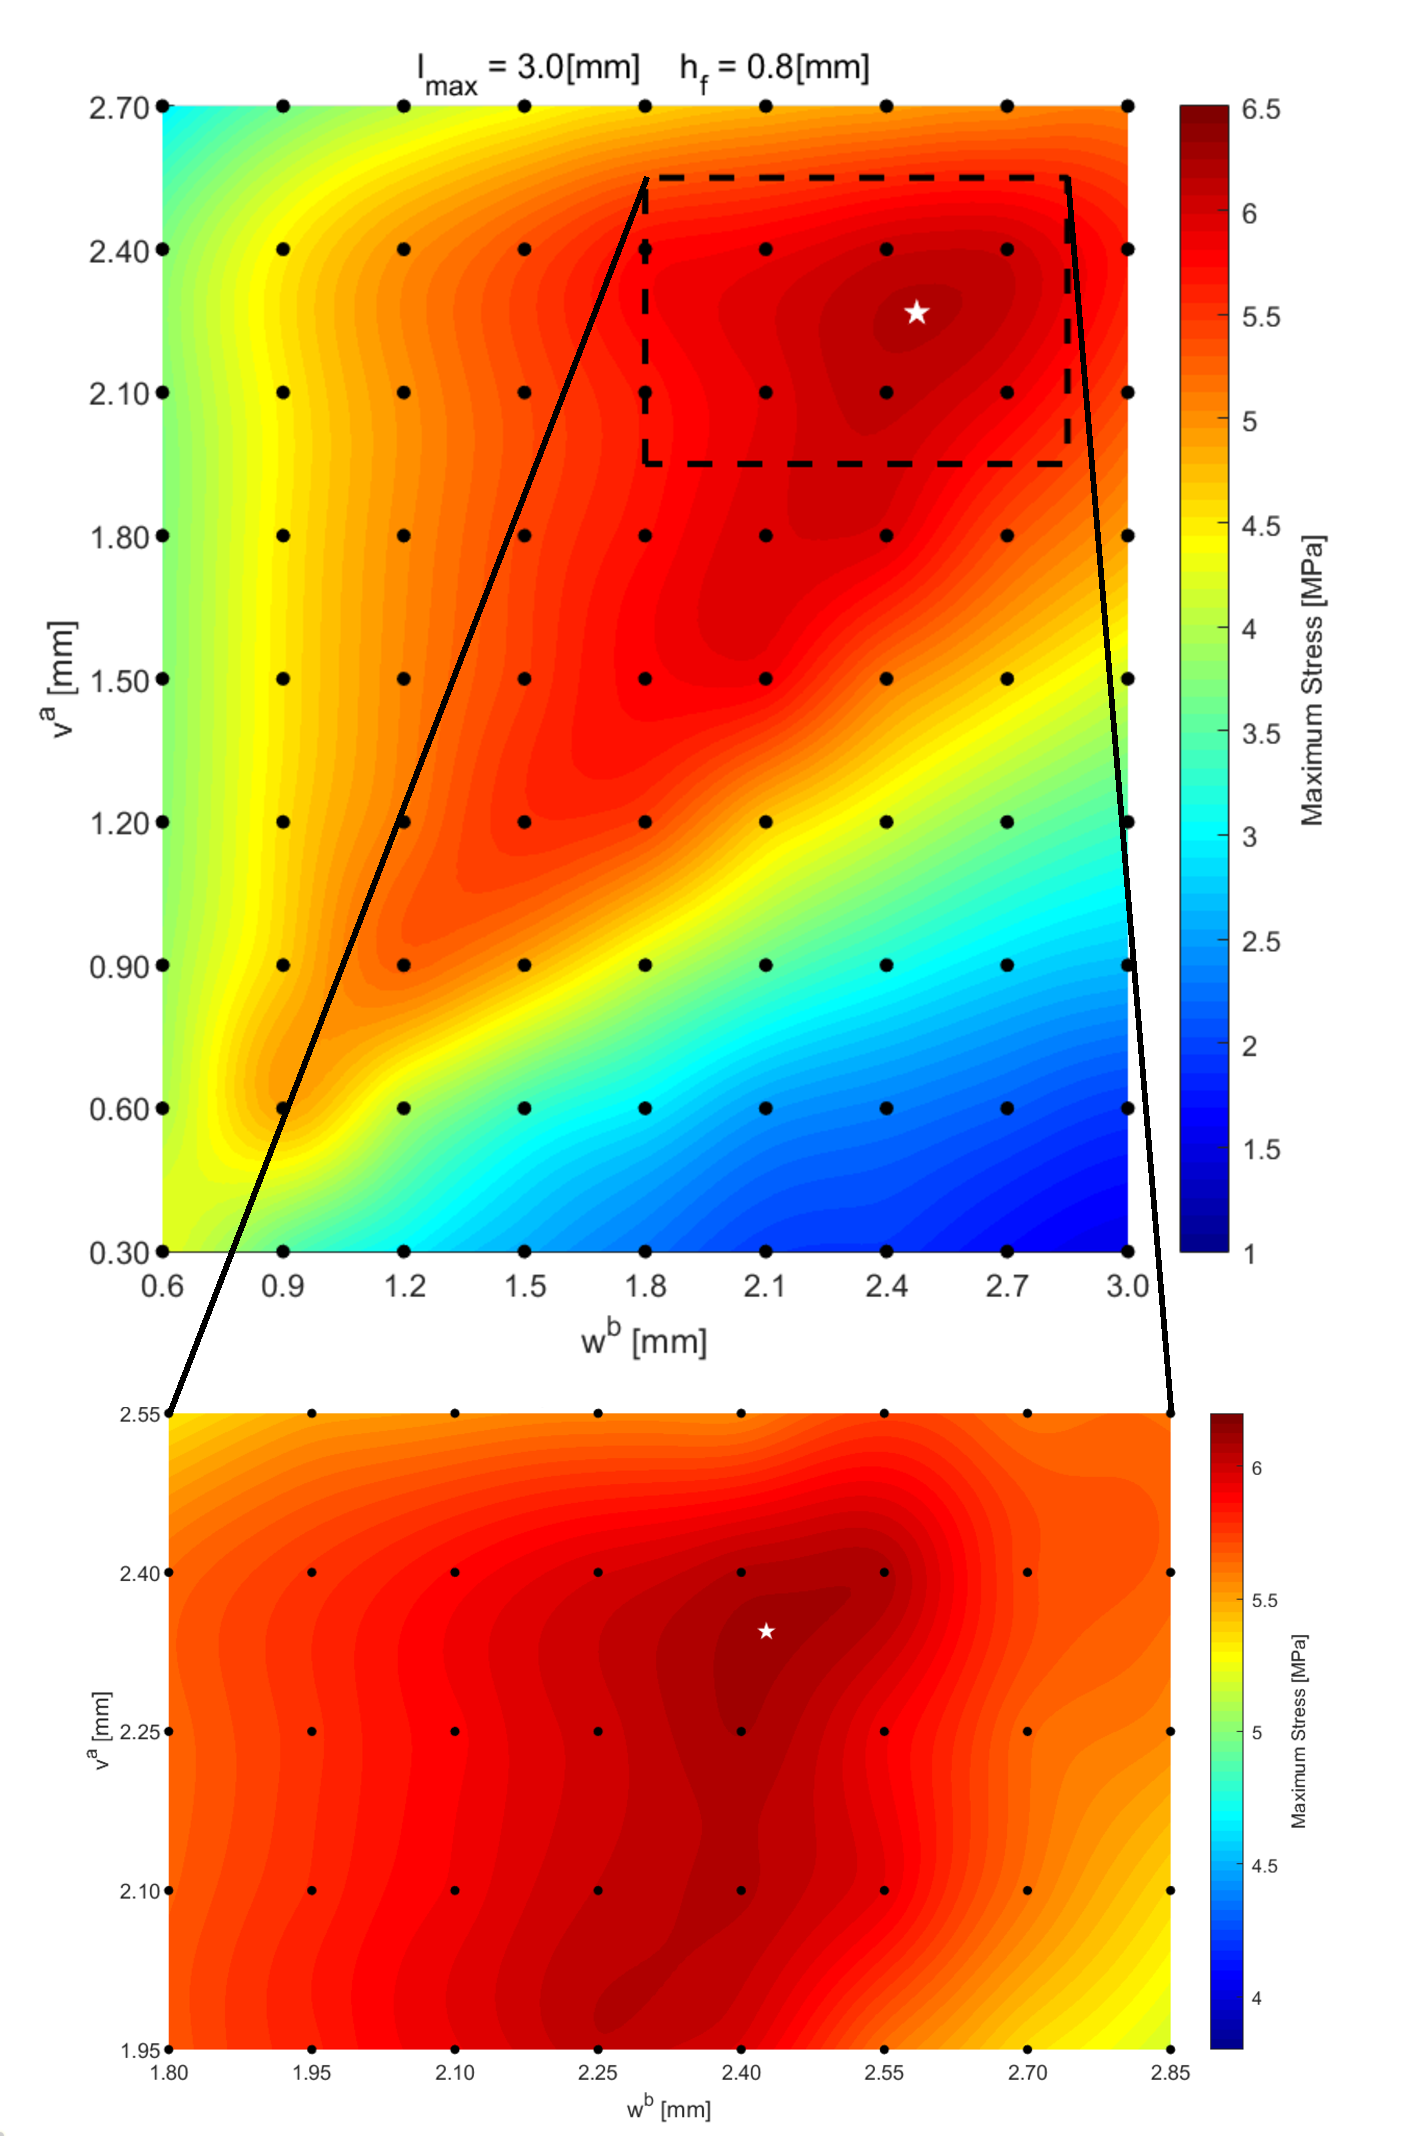
\includegraphics{sources/simulation/r12-lmax3.0.pdf}
		\caption{$\lmax=\SI{3.0}{\milli\meter}; \hf=\SI{0.8}{\milli\meter}$}
	\end{subfigure}
	\begin{subfigure}[B]{.49\columnwidth}
		\centering
		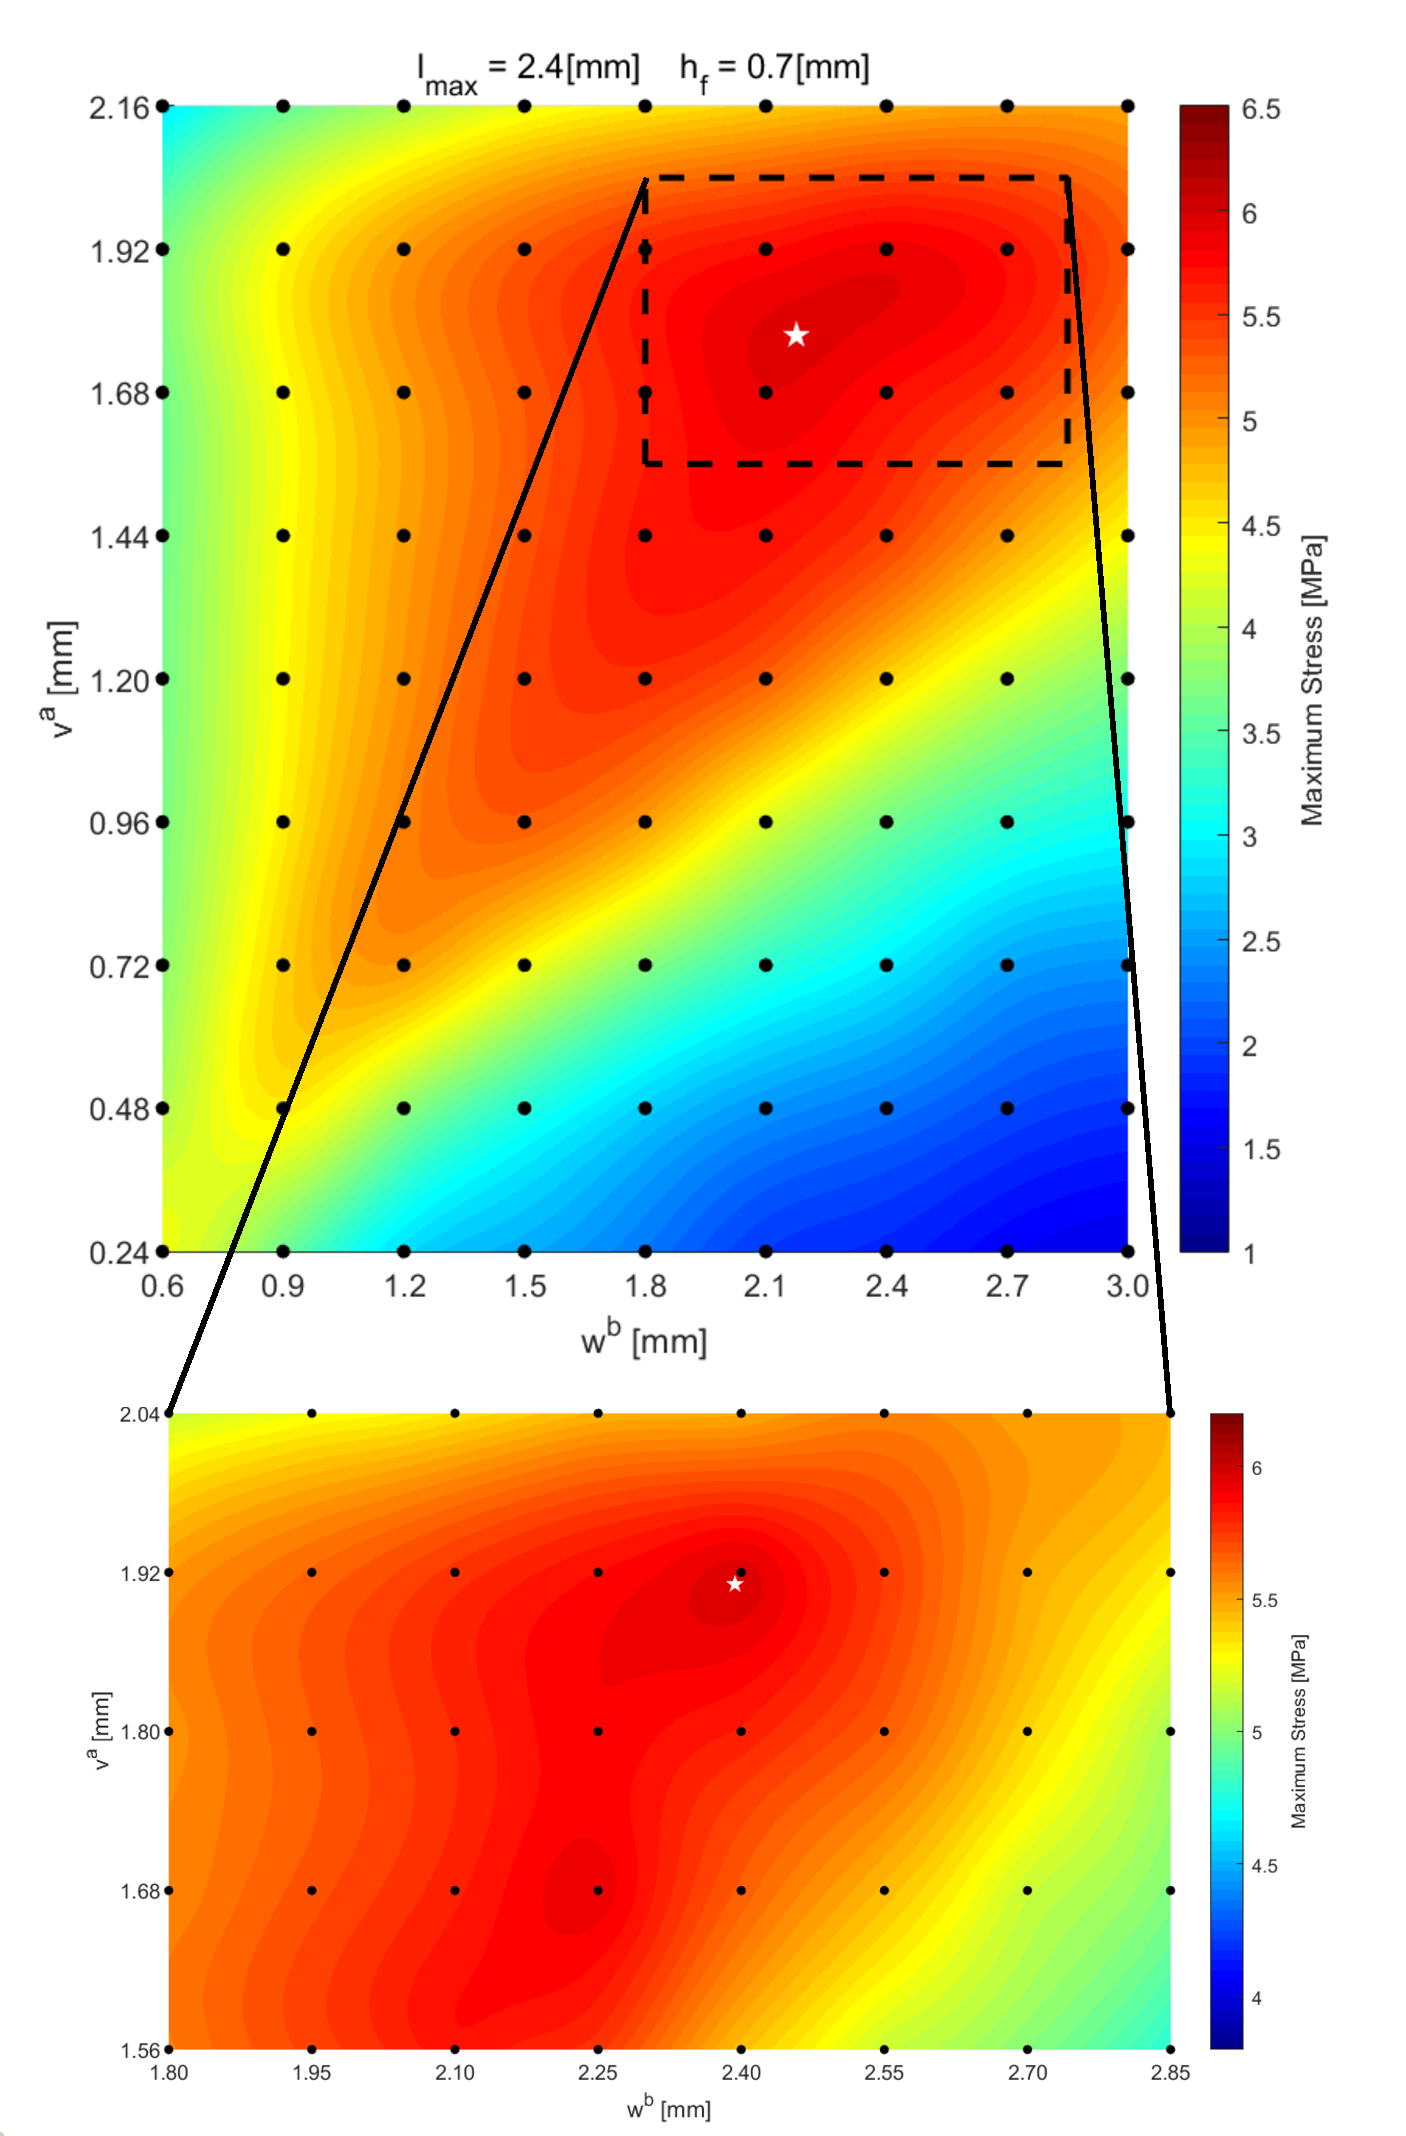
\includegraphics{sources/simulation/r12-lmax2.4.pdf}
		\caption{$\lmax=\SI{2.4}{\milli\meter}; \hf=\SI{0.7}{\milli\meter}$}
	\end{subfigure}
	\begin{subfigure}[B]{.49\columnwidth}
		\centering
		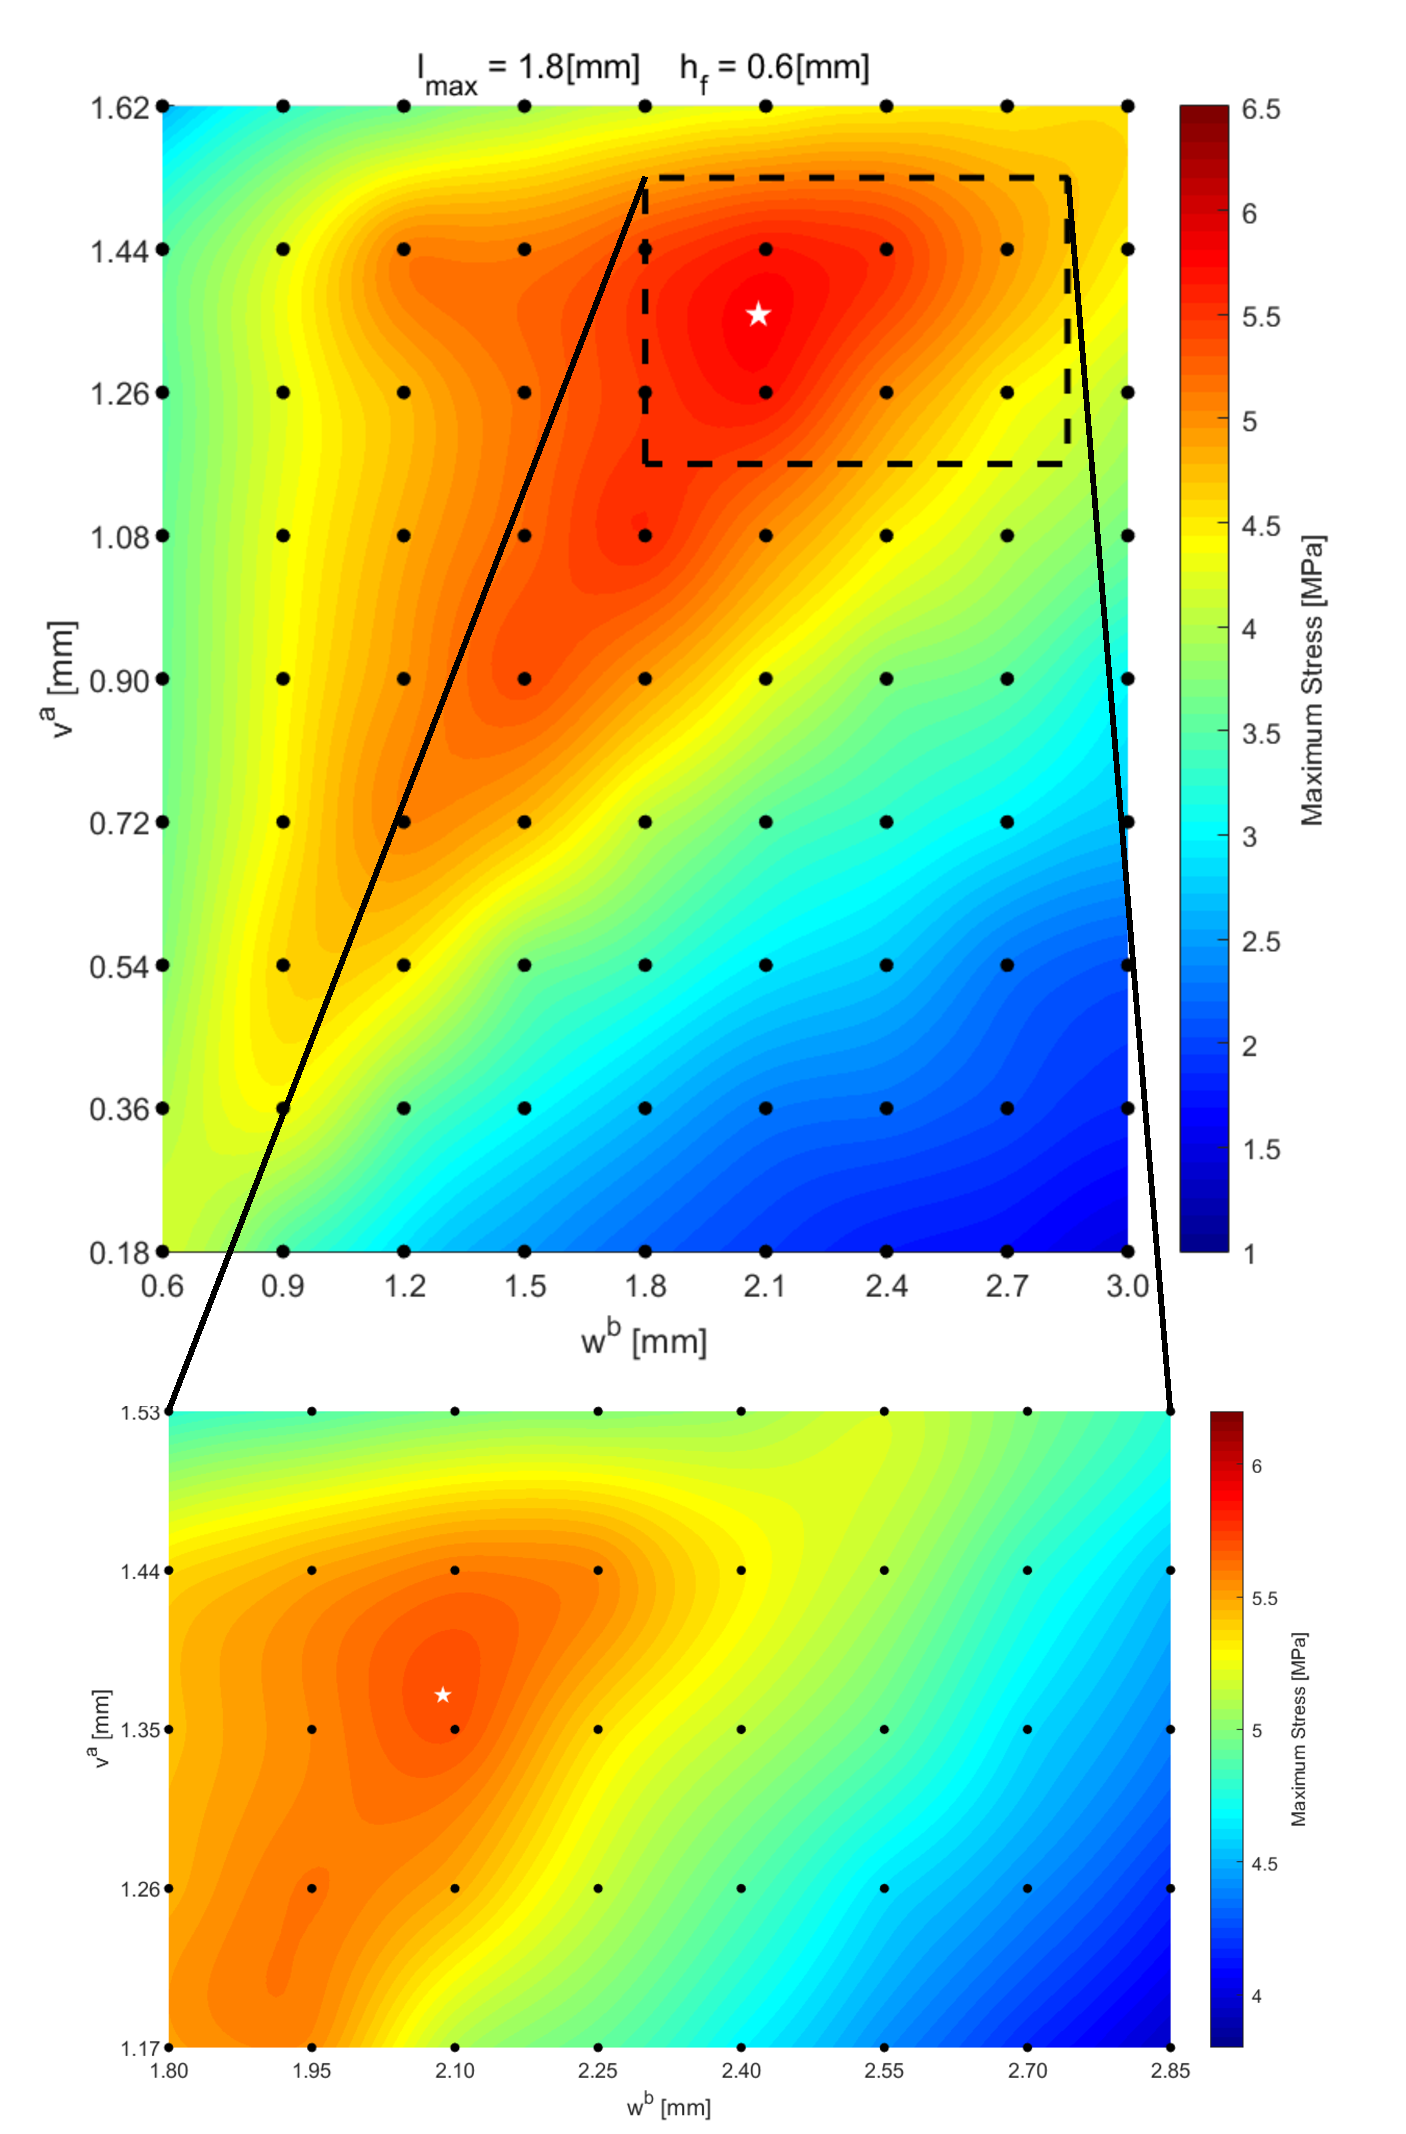
\includegraphics{sources/simulation/r12-lmax1.8.pdf}
		\caption{$\lmax=\SI{1.8}{\milli\meter}; \hf=\SI{0.6}{\milli\meter}$}
	\end{subfigure}
	\caption{2D slices of the 4D simulation results and fitted hypersurface for the straight design.}
	\label{fig:simulation_results_straight}
\end{figure*}

\begin{table}
	\caption{Optimal designs according to the hypersurface fitted to the second round of FEM simulations.}
	\label{tab:sim_straight_optima}
	\begin{tabular}{l|llll}
		$\lmax$ (\si{\milli\meter})             & 3.6 & 3.0 & 2.4 & 1.8 \\
		\hline
		$\sigma_\text{max}$ (\si{\mega\pascal}) & \bf 6.11 & \bf 6.03 & \bf 5.81 & \bf 5.53 \\
		$\hf$ (\si{\milli\meter})               & 0.8 & 0.8 & 0.7 & 0.6 \\
		$\wb$ (\si{\milli\meter})               & 2.54 & 2.35 & 2.22 & 2.01 \\
		$\va$ (\si{\milli\meter})               & 2.82 & 2.27 & 1.84 & 1.36
		\end
		{tabular}
\iffalse
	\begin{tabular}{l|llllllll}
		Round & 1 & 2 & 1 & 2 & 1 & 2 & 1 & 2 \\
		\hline
		$\lmax$ (\si{\milli\meter}) & 3.6 & 3.6 & 3.0 & 3.0 & 2.4 & 2.4 & 1.8 & 1.8\\
		$\hf$ (\si{\milli\meter}) & 0.8 & 0.8 & 0.8 & 0.8 & 0.7 & 0.7 & 0.6 & 0.6 \\
		$\wb$ (\si{\milli\meter}) & 2.58 & 2.54 & 2.42 & 2.35 & 2.18 & 2.22 & 2.05 & 2.01\\
		$\va$ (\si{\milli\meter}) & 2.67 & 2.82 & 2.23 & 2.27 & 1.78 & 1.84 & 1.35 & 1.36 \\
		$\sigma_\text{max}$ (\si{\mega\pascal}) & 6.17 & 6.11 & 6.12 & 6.03 & 5.89 & 5.81 & 5.59 & 5.53
	\end{tabular}
\fi
\end{table}



\subsection{Diagonal}
results





